\Transcb{yellow}{blue}{Link with cosmic rays}
\onecolumn

\begin{itemize}
\item Assume UHECR fluence originates from GRBs~:
      $\displaystyle S_{obs}=\frac{E_{cr}}{4\pi (r_{phys})^{2}(1+z)}$\\[1mm]
\item Spherical shell of thickness $\d r \rightarrow \d N=n \cdot 4\pi r_{phys}^{2} \d r$ GRBs per year
\item CR flux observed on earth originating from this shell~:
      $\displaystyle F_{shell}(r)=S\,dN=\frac{E_{cr}n\,\d r}{1+z}$
\item Total CR flux observed on earth~:
      $\displaystyle F_{cr}=\int_{r=0}^{r_{max}} \frac{E_{cr}n\,\d r}{1+z}$
\item Simplified model for $r_{phys}(z) \rightarrow$
      $\displaystyle F_{cr}=\int_{0}^{\infty} \frac{c E_{cr} n \, \d z}{H_{0}(1+z)^{3/2}}
       =\frac{2cE_{cr}n}{3H_{0}}$
\item Taking $E_{cr}=10^{52}$ erg $\quad n=1.7 \cdot 10^{-10}$ Mpc$^{-3}$ yr$^{-1}$
\item[] $\rightarrow F_{cr} \approx 10^{-8}$ GeV cm$^{-2}$ s$^{-1} \quad$
        (observed $\approx 10^{-7}$ GeV cm$^{-2}$ s$^{-1}$)
\item[] Not a bad result for a simplified model !
\end{itemize}

\begin{center}
\colorbox{yellow}{What sort of particles could these be and where do they come from~?}
\end{center}

\Tr
\onecolumn
\begin{center}
{\blue It's a long and difficult journey}\\[5mm]
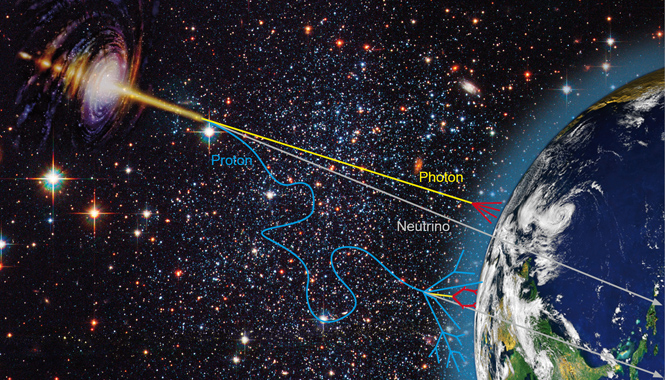
\includegraphics[keepaspectratio,height=13cm]{app}\\[5mm]
\colorbox{yellow}{Only photons and neutrinos point back to the source}
\end{center}

\Tr
\onecolumn
\begin{center}
{\blue Beware of the observable Universe:
 $\gamma+\gamma_{EBL}\rightarrow e^{+}e^{-} \qquad N+\gamma_{CMB} \rightarrow \Delta$}\\
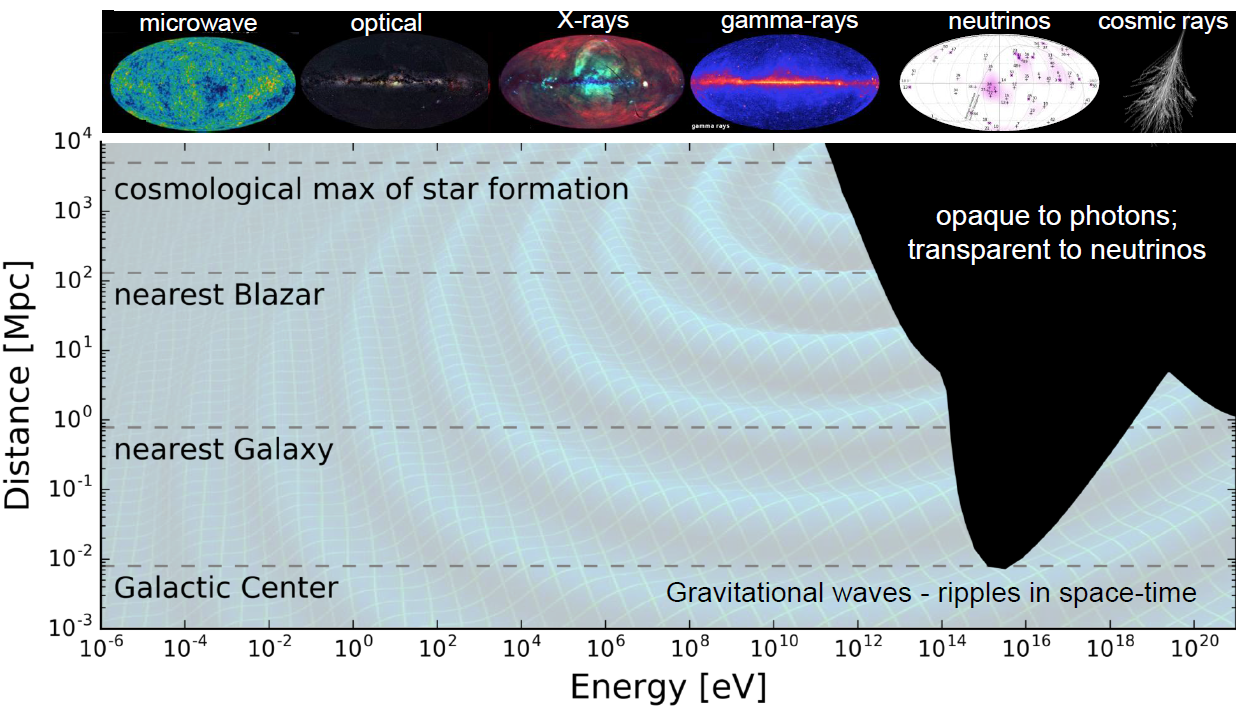
\includegraphics[keepaspectratio,height=14cm]{marek}\\
{\large [Credit Marek Kowalski]}
\end{center}

\twocolumn
